\subsection{Entrega del sistema ViaData — Medellín}

El desarrollo culminó en una plataforma web funcional que integra backend Django con API REST, base PostgreSQL/PostGIS y frontend React. Los módulos entregados cubren mapa analítico (\texttt{/}, \texttt{/mapa}), tablero de indicadores (\texttt{/tablero}), predicciones (\texttt{/predicciones}), reportes imprimibles (\texttt{/reporte/vista}), asistente conversacional (\texttt{/agente}) y gestión de usuarios (\texttt{/admin/usuarios}), con autenticación JWT y roles diferenciados (ciudadano, analista, administrador). El módulo de predicciones fue evaluado y cerrado el 18 de junio de 2026 con evidencia reproducible en archivos CSV y scripts de evaluación.

\subsection{Cumplimiento de objetivos}

La Tabla~\ref{tab:cumplimiento-objetivos} relaciona los objetivos planteados con la evidencia observable en el sistema. Los componentes complementarios (mapa, reportes, asistente y administración de usuarios) se reportan como entregables de apoyo, sin ampliar la formulación original de objetivos.

\begin{table}[H]
	\centering
	\caption{Cumplimiento de objetivos y componentes de ViaData — Medellín}
	\label{tab:cumplimiento-objetivos}
	\small
	\begin{tabularx}{\linewidth}{@{}l X c@{}}
		\toprule
		\textbf{Elemento} & \textbf{Evidencia en el sistema} & \textbf{Estado} \\
		\midrule
		Objetivo general & Instrumento geoespacial con visualización, análisis, segmentación y modelos estadísticos orientativos & Cumplido \\
		OE1: arquitectura y modelo de datos & Monolito Django + PostGIS; ETL \texttt{mede\_limpieza.py}; entidades incidente/víctima/catálogos & Cumplido \\
		OE2: módulos de análisis estadístico & KPIs, rankings, índice P05, proyecciones §1--§5, densidad y hotspots & Cumplido \\
		OE3: tablero de monitoreo & Series mensuales, matrices día$\times$hora, filtros territoriales y temporales & Cumplido \\
		OE4: validación técnica & Suite \texttt{pytest} en apps críticas; consultas PostGIS verificables & Cumplido \\
		Mapa analítico (complementario) & Puntos, heatmap, coroplética, G03, modo registro/espacial & Entregado \\
		Reportes y asistente (complementarios) & Exportación imprimible; Gemini con herramientas sobre la API & Entregado \\
		\bottomrule
	\end{tabularx}
\end{table}

\subsection{Carga de datos y calidad de la base}

Tras el pipeline ETL documentado, la base operativa concentra registros Mede entre \textbf{2014-01-01} y \textbf{2021-09-30}, con del orden de \textbf{160\,000+} incidentes con coordenadas válidas. En el escenario de referencia A (2018--2021, exclusión COVID en el ajuste), el periodo filtrado para priorización territorial registra \textbf{75\,088} incidentes a nivel ciudad y \textbf{22} comunas elegibles.

El indicador \textbf{G03} cuantifica la coincidencia entre el territorio declarado en el registro Mede y el asignado espacialmente por polígono oficial. En modo espacial PostGIS, el escenario A de prioridad territorial reporta \textbf{66\,137} incidentes con \textbf{21} comunas elegibles, lo que permite contrastar la lectura administrativa frente a la cartográfica. La depuración centralizada en \texttt{mede\_limpieza.py} asegura coherencia entre el análisis exploratorio, la carga a PostgreSQL y los cálculos expuestos en la interfaz.

\subsection{Resultados descriptivos y geoespaciales}

El tablero y el mapa materializan la analítica descriptiva y diagnóstica sobre el periodo y los filtros seleccionados por el usuario. La Figura~\ref{fig:captura-tablero} muestra los KPIs del escenario de referencia (ciudad completa, 2018--2021): \textbf{75\,088} incidentes ($-2{,}69\,\%$ frente al año anterior), \textbf{108\,541} víctimas y \textbf{703} fatales ($+1{,}01\,\%$). Entre los hallazgos recurrentes destacan:

\begin{itemize}
	\item \textbf{Concentración territorial:} La Candelaria encabeza rankings por volumen en múltiples cortes (75\,088 incidentes ciudad; 12\,921 en La Candelaria en escenario A de prioridad).
	\item \textbf{Patrón temporal:} La celda líder día$\times$hora histórica es \textbf{martes 07:00}; el día con mayor participación relativa es \textbf{martes} (patrones P12/P13, escenario A).
	\item \textbf{Gravedad relativa:} El porcentaje mensual observado de víctimas fatales en ciudad se sitúa en torno a \textbf{0,66\,\%} (rango 0,35--1,2\,\%), con variabilidad mensual elevada.
	\item \textbf{Calidad espacial:} El modo registro frente al modo espacial produce rankings comparables en comunas (Spearman índice$\leftrightarrow$frecuencia $\approx 0{,}86$ en modo espacial), útil para discutir la confiabilidad cartográfica del dato \cite{monar2025}.
\end{itemize}

\begin{figure}[H]
	\centering
	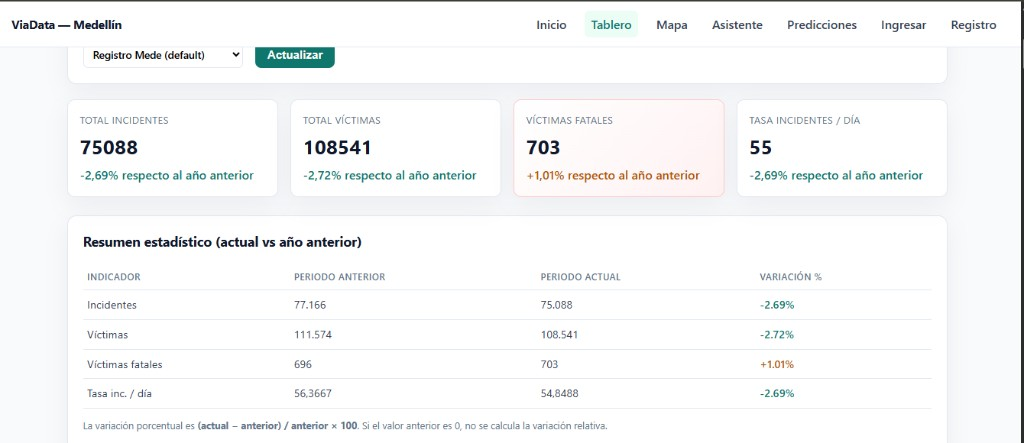
\includegraphics[width=0.92\linewidth]{images/captura_tablero.png}
	\caption{Tablero de indicadores — KPIs y resumen estadístico (ciudad completa, 2018--2021)}
	\label{fig:captura-tablero}
\end{figure}

La Figura~\ref{fig:captura-mapa-densidad} ilustra la capa de \textbf{densidad territorial} (G01--G02) en el mapa analítico para el periodo 2021-01-01 — 2021-09-30, con coroplética por comunas. La concentración en el valle urbano central ---La Candelaria, Laureles-Estadio, Robledo y corredores adyacentes--- es coherente con los rankings del tablero y del índice P05.

\begin{figure}[H]
	\centering
	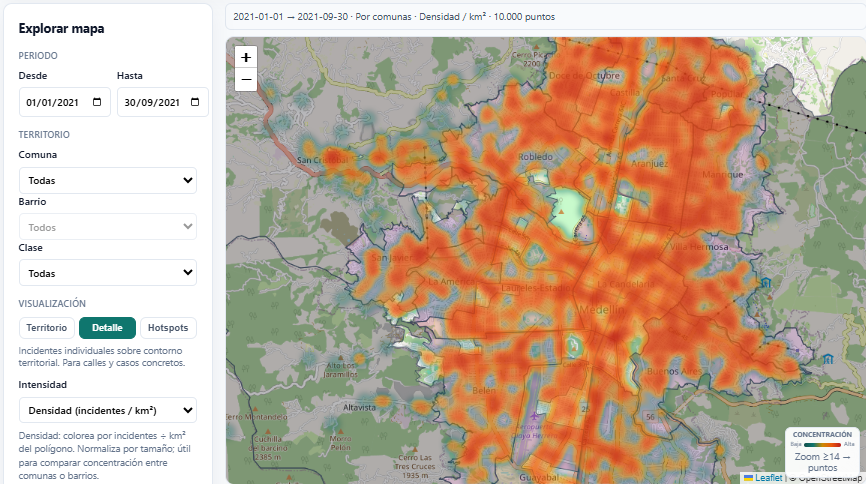
\includegraphics[width=0.88\linewidth]{images/captura_mapa_densidad.png}
	\caption{Mapa analítico — densidad de incidentes por km$^2$ (ene.--sep. 2021, por comunas)}
	\label{fig:captura-mapa-densidad}
\end{figure}

Estos resultados alimentan la priorización territorial (§2) y contextualizan las proyecciones del módulo predictivo.

\subsection{Evaluación del módulo de predicciones}

La evaluación siguió el protocolo metodológico: hold-out de 3 meses, exclusión por defecto de mar--ago 2020 en el ajuste y umbral exploratorio de MAPE hold-out $\leq 20\,\%$. Las tablas siguientes sintetizan los hallazgos principales; el detalle completo permanece en los CSV de \texttt{Fuentes\_viaData/}.

\subsubsection{§1 — Proyección mensual}

En el escenario A (ciudad completa, incidentes, 2018--2021), la Tabla~\ref{tab:resultados-seccion1-a} compara los siete modelos evaluados. \textbf{SARIMA}$(2,1,3)(1,1,1)_{12}$ obtiene el menor MAPE hold-out (\textbf{12,62\,\%}, precisión estimada $\approx 87{,}4\,\%$), por debajo de Poisson y estacional pese a un MAPE in-sample más alto en estos últimos. Este resultado confirma que el criterio hold-out evita sobreajuste: modelos que ajustan bien in-sample no necesariamente generalizan mejor.

\begin{table}[H]
	\centering
	\caption{Proyección mensual de incidentes — escenario A (hold-out 3 meses)}
	\label{tab:resultados-seccion1-a}
	\small
	\begin{tabularx}{\linewidth}{@{}l r r r c@{}}
		\toprule
		\textbf{Modelo} & \textbf{MAPE in-sample (\%)} & \textbf{MAPE hold-out (\%)} & \textbf{Prec. est. (\%)} & \textbf{$\geq 80\,\%$} \\
		\midrule
		SARIMA & 13,14 & \textbf{12,62} & $\approx$87,4 & Sí \\
		Media móvil (3 m) & 6,52 & 15,71 & $\approx$84,3 & Sí \\
		$\mu \pm 3\sigma$ & 11,25 & 17,19 & $\approx$82,8 & Sí \\
		OLS & 11,21 & 18,92 & $\approx$81,1 & Sí \\
		ARIMA & 10,95 & 19,90 & $\approx$80,1 & Límite \\
		Poisson & 8,30 & 22,54 & $\approx$77,5 & No \\
		Estacional & 8,38 & 22,44 & $\approx$77,6 & No \\
		\bottomrule
	\end{tabularx}
\end{table}

La Tabla~\ref{tab:resultados-seccion1-escenarios} resume el mejor modelo por escenario representativo. Para víctimas a nivel ciudad (B) destaca media móvil (14,67\,\%); para víctimas fatales (C), estacional (19,67\,\%); en Castilla (D), media móvil (8,42\,\%); en atropellos (E), Poisson (11,64\,\%). El escenario F, que \textbf{no excluye} COVID del ajuste, degrada SARIMA a 32,87\,\% de MAPE hold-out, reforzando la decisión de exclusión por defecto en la interfaz.

\begin{table}[H]
	\centering
	\caption{Mejor modelo por escenario en proyección mensual (§1)}
	\label{tab:resultados-seccion1-escenarios}
	\small
	\begin{tabularx}{\linewidth}{@{}c l l r@{}}
		\toprule
		\textbf{ID} & \textbf{Contexto} & \textbf{Mejor modelo} & \textbf{MAPE hold-out (\%)} \\
		\midrule
		A & Incidentes ciudad & SARIMA & 12,62 \\
		B & Víctimas ciudad & Media móvil & 14,67 \\
		C & Víctimas fatales ciudad & Estacional & 19,67 \\
		D & Comuna Castilla & Media móvil & 8,42 \\
		E & Clase atropello & Poisson & 11,64 \\
		F & Sin excluir COVID & OLS (11,72); SARIMA (32,87) & Confirma excluir COVID \\
		\bottomrule
	\end{tabularx}
\end{table}

\textbf{Decisión adoptada:} SARIMA$(2,1,3)(1,1,1)_{12}$ para incidentes ciudad; media móvil de tres meses como alternativa interpretable.

Las Figuras~\ref{fig:captura-sarima} y \ref{fig:captura-estacional} muestran la misma configuración de filtros en la interfaz (2018--2021, incidentes ciudad, exclusión mar--ago 2020, hold-out 3 meses) con dos modelos distintos. SARIMA exhibe MAPE hold-out de 12,62\,\% ($\approx 87{,}4\,\%$ de precisión estimada) pese a R$^2$ in-sample bajo; el estacional mejora el ajuste histórico (MAPE 8,38\,\%) pero pierde en la prueba reservada (22,44\,\%), ilustrando por qué la plataforma compara modelos bajo el mismo escenario antes de adoptar uno por defecto.

\begin{figure}[H]
	\centering
	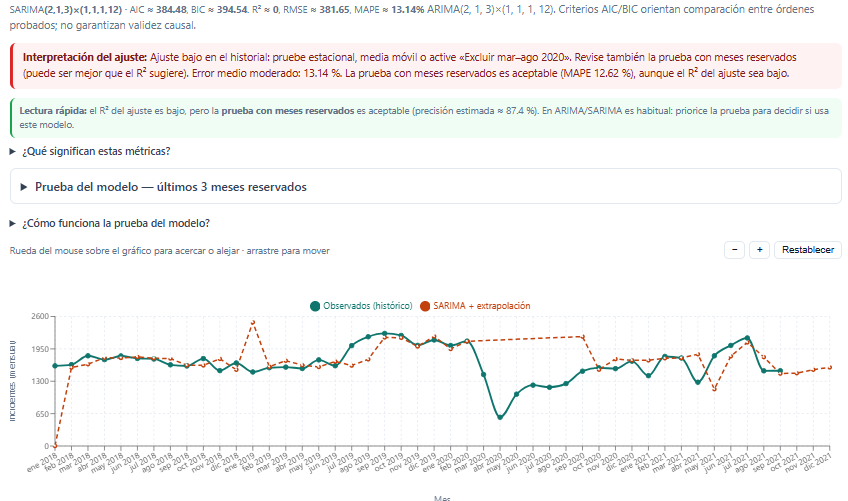
\includegraphics[width=0.92\linewidth]{images/captura_predicciones_sarima.png}
	\caption{Proyección mensual §1 — SARIMA$(2,1,3)(1,1,1)_{12}$, escenario A (hold-out 3 meses)}
	\label{fig:captura-sarima}
\end{figure}

\begin{figure}[H]
	\centering
	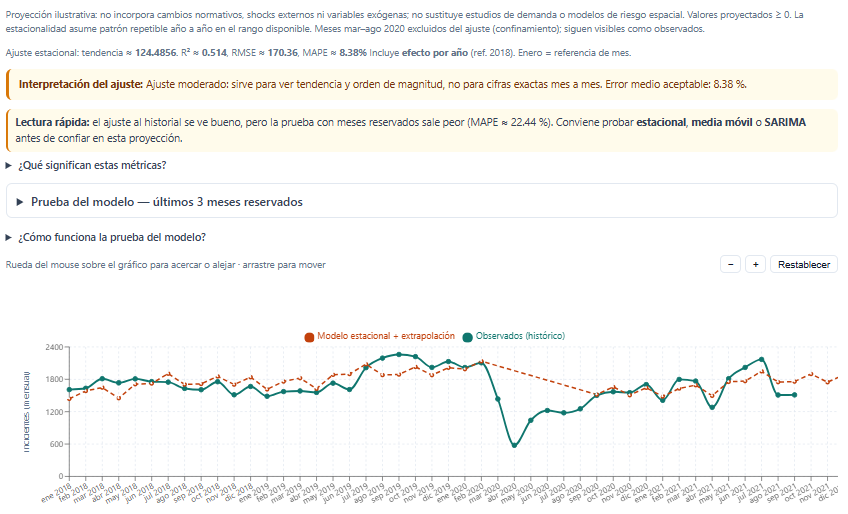
\includegraphics[width=0.92\linewidth]{images/captura_predicciones_estacional.png}
	\caption{Proyección mensual §1 — modelo estacional, mismo escenario A (contraste hold-out)}
	\label{fig:captura-estacional}
\end{figure}

\subsubsection{§2 — Prioridad territorial (índice P05)}

El índice multicriterio P05 (30/15/20/20/15) no entrena modelos predictivos: ordena territorios del periodo filtrado. En escenario A (comunas), \textbf{La Candelaria} lidera con índice \textbf{62,6} y 12\,921 incidentes; la correlación de Spearman entre índice y frecuencia es \textbf{0,8498} y el solapamiento top-5 índice/frecuencia es de 5 territorios, calificando el ranking como \textbf{útil} para priorización. La Figura~\ref{fig:captura-p05} reproduce el ranking en la interfaz, donde La Candelaria lidera por frecuencia, densidad y participación (scores 100 en esos componentes). En barrios (escenario B), el líder por índice es Sin Inf (Robledo), pero el ranking se marca \textbf{parcial} porque el \#1 por índice no coincide con el \#1 por volumen (Spearman 0,9033 sobre top 50 de 270 barrios).

\begin{figure}[H]
	\centering
	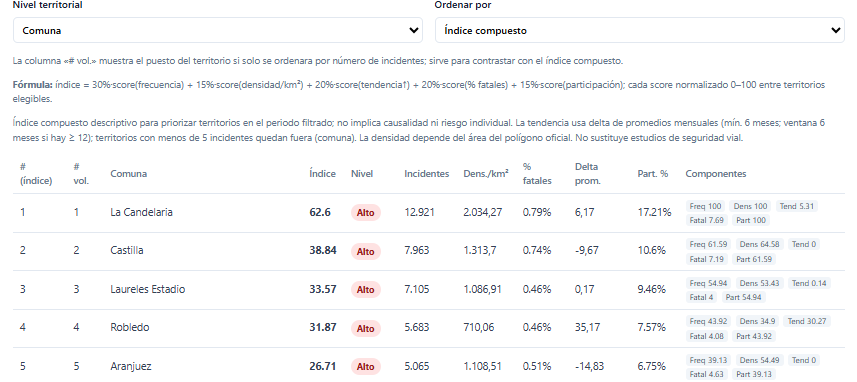
\includegraphics[width=0.95\linewidth]{images/captura_prioridad_p05.png}
	\caption{Prioridad territorial §2 — índice P05 por comuna (escenario A, 2018--2021)}
	\label{fig:captura-p05}
\end{figure}

\subsubsection{§3 — Carga territorial}

En escenario A (comunas), el modelo \textbf{estacional} proyecta la mayor carga en \textbf{La Candelaria} (982,2 incidentes en horizonte de 3 meses) con Spearman carga$\leftrightarrow$frecuencia de \textbf{0,9492} y coherencia con P05 en el territorio líder. El MAPE mediano hold-out territorial ronda \textbf{33\,\%}: las cifras absolutas deben leerse de forma \textbf{comparativa}, no como presupuesto exacto. ARIMA desplaza el líder a Sin Inf (cierre \textbf{parcial}). A nivel barrio, 220 de 270 territorios carecen de proyección individual en el ajuste, por lo que el ranking ciudadano por barrio se reporta como \textbf{parcial}.

\subsubsection{§4 — Proporción de víctimas fatales}

Para el porcentaje mensual de víctimas fatales (escenario A), el modelo \textbf{estacional} alcanza MAPE hold-out de \textbf{21,96\,\%} con R$^2 = 0{,}38$; \textbf{logit con exposición} (20,25\,\%) y \textbf{ratio compuesto} (21,18\,\%) son alternativas viables. OLS, logística, media móvil y ARIMA/SARIMA superan el umbral del 20\,\% en hold-out o presentan R$^2$ cercano a cero, coherente con la volatilidad del indicador. El porcentaje proyectado en horizonte se sitúa en torno a \textbf{0,67\,\%}, cercano al promedio histórico.

\begin{table}[H]
	\centering
	\caption{Proporción de víctimas fatales — escenario A (hold-out 3 meses)}
	\label{tab:resultados-seccion4-a}
	\small
	\begin{tabularx}{\linewidth}{@{}l r r r c@{}}
		\toprule
		\textbf{Modelo} & \textbf{R$^2$} & \textbf{MAPE ajuste (\%)} & \textbf{MAPE hold-out (\%)} & \textbf{Útil} \\
		\midrule
		Estacional & 0,38 & 16,46 & \textbf{21,96} & Sí \\
		Logit con exposición & 0,36 & 15,23 & 20,25 & Sí \\
		Ratio compuesto & 0,38 & 16,13 & 21,18 & Sí \\
		Media móvil & 0,32 & 17,01 & 35,09 & No \\
		OLS / logística & $\approx 0$ & $>$21 & $>$35 & No \\
		\bottomrule
	\end{tabularx}
\end{table}

\subsubsection{§5 — Patrones temporales (P12 y P13)}

Los patrones día$\times$hora heredan el total proyectado de §1 y reparten según pesos históricos con suavizado Laplace. En escenario A, con modelo estacional en §1, el total proyectado a 3 meses es \textbf{5\,530,96} incidentes; la celda líder \textbf{P12} permanece en \textbf{martes 07:00} (69 incidentes proyectados, 1,25\,\% de participación) y el día líder \textbf{P13} es \textbf{martes} (842 incidentes, 15,22\,\%). El Spearman entre ranking observado y proyectado de celdas alcanza \textbf{0,9992}: los modelos mensuales alteran el volumen total pero \textbf{no cambian el patrón relativo} de concentración horaria. Con SARIMA adoptado en §1, el total baja a 4\,572,92 incidentes, manteniendo los mismos líderes temporales.

\subsubsection{Evaluación complementaria $\mu \pm 3\sigma$}

El modelo de línea base $\mu \pm 3\sigma$ proyecta la media histórica con bandas de control. En escenario A (§1), la media es 1\,753,4 incidentes/mes ($\sigma = 247{,}6$); el 100\,\% de los meses de ajuste caen dentro de $\mu \pm 3\sigma$ y el MAPE hold-out es 17,19\,\%. No reemplaza a SARIMA en ciudad, pero aporta un contraste didáctico y bandas de control interpretables.

\subsection{Validación técnica del software}

La validación técnica se ejecutó mediante la suite \texttt{pytest} con \texttt{pytest-django} sobre las aplicaciones \texttt{dashboard}, \texttt{agent}, \texttt{accounts} y \texttt{reports}, usando configuración de prueba con SQLite en memoria. La ejecución completa finalizó en verde, cubriendo endpoints de KPIs, predicciones, autenticación JWT, herramientas del asistente y generación de payloads de reportes. Complementariamente, el comando \texttt{manage.py check\_postgis} verifica la disponibilidad de extensiones espaciales en despliegues con PostgreSQL.

Esta evidencia respalda el objetivo específico de validar desempeño y seguridad del software. No sustituye una auditoría de carga en producción, pero confirma que los módulos críticos del backend responden de forma coherente bajo pruebas automatizadas reproducibles.

\subsection{Síntesis de resultados}

En conjunto, ViaData — Medellín cumple los objetivos planteados y entrega un instrumento geoespacial consultable sobre datos Mede. La analítica descriptiva identifica concentraciones territoriales y temporales estables (La Candelaria; martes 07:00). El módulo predictivo adopta modelos transparentes con validación hold-out: SARIMA para incidentes ciudad, estacional para carga territorial y proporción de fatales, e índice P05 fijo para priorización inmediata. Las limitaciones de precisión territorial (MAPE mediano $\approx 33\,\%$), la volatilidad del \% de fatales y el alcance parcial en barrios se discuten en la sección de discusión.
